%% This is file `sample-sigconf-authordraft.tex',
%% generated with the docstrip utility.
%%
%% The original source files were:
%%
%% samples.dtx  (with options: `all,proceedings,bibtex,authordraft')
%% 
%% IMPORTANT NOTICE:
%% 
%% For the copyright see the source file.
%% 
%% Any modified versions of this file must be renamed
%% with new filenames distinct from sample-sigconf-authordraft.tex.
%% 
%% For distribution of the original source see the terms
%% for copying and modification in the file samples.dtx.
%% 
%% This generated file may be distributed as long as the
%% original source files, as listed above, are part of the
%% same distribution. (The sources need not necessarily be
%% in the same archive or directory.)
%%
%%
%% Commands for TeXCount
%TC:macro \cite [option:text,text]
%TC:macro \citep [option:text,text]
%TC:macro \citet [option:text,text]
%TC:envir table 0 1
%TC:envir table* 0 1
%TC:envir tabular [ignore] word
%TC:envir displaymath 0 word
%TC:envir math 0 word
%TC:envir comment 0 0
%%
%%
%% The first command in your LaTeX source must be the \documentclass
%% command.
%%
%% For submission and review of your manuscript please change the
%% command to \documentclass[manuscript, screen, review]{acmart}.
%%
%% When submitting camera ready or to TAPS, please change the command
%% to \documentclass[sigconf]{acmart} or whichever template is required
%% for your publication.
%%
%%
%\documentclass[manuscript, screen, review]{acmart}
\documentclass[sigconf,authordraft]{acmart}

%%
%% \BibTeX command to typeset BibTeX logo in the docs
\AtBeginDocument{%
  \providecommand\BibTeX{{%
    Bib\TeX}}}

%% Rights management information.  This information is sent to you
%% when you complete the rights form.  These commands have SAMPLE
%% values in them; it is your responsibility as an author to replace
%% the commands and values with those provided to you when you
%% complete the rights form.
\setcopyright{acmlicensed}
\copyrightyear{2024}
\acmYear{2024}
\acmDOI{XXXXXXX.XXXXXXX}

%% These commands are for a PROCEEDINGS abstract or paper.
%\acmConference[Conference acronym 'XX]{Make sure to enter the correct conference title from your rights confirmation emai}{June 03--05, 2018}{Woodstock, NY}
%%
%%  Uncomment \acmBooktitle if the title of the proceedings is different
%%  from ``Proceedings of ...''!
%%
%%\acmBooktitle{Woodstock '18: ACM Symposium on Neural Gaze Detection,
%%  June 03--05, 2018, Woodstock, NY}
\acmISBN{978-1-4503-XXXX-X/18/06}
%%
%% Submission ID.
%% Use this when submitting an article to a sponsored event. You'll
%% receive a unique submission ID from the organizers
%% of the event, and this ID should be used as the parameter to this command.
%%\acmSubmissionID{123-A56-BU3}

%%
%% For managing citations, it is recommended to use bibliography
%% files in BibTeX format.
%%
%% You can then either use BibTeX with the ACM-Reference-Format style,
%% or BibLaTeX with the acmnumeric or acmauthoryear sytles, that include
%% support for advanced citation of software artefact from the
%% biblatex-software package, also separately available on CTAN.
%%
%% Look at the sample-*-biblatex.tex files for templates showcasing
%% the biblatex styles.
%%

%%
%% The majority of ACM publications use numbered citations and
%% references.  The command \citestyle{authoryear} switches to the
%% "author year" style.
%%
%% If you are preparing content for an event
%% sponsored by ACM SIGGRAPH, you must use the "author year" style of
%% citations and references.
%% Uncommenting
%% the next command will enable that style.
%%\citestyle{acmauthoryear}

\title{Towards Greener Networks: A Statistical \\ Approach to RAN Cell Control}
\author{Anonymous Authors}
\usepackage[english]{babel}
\usepackage{xspace}
\usepackage[normalem]{ulem}
\useunder{\uline}{\ul}{}


\usepackage{tabularx,colortbl}
\newcolumntype{Y}{>{\centering\arraybackslash}X}
\def\tabularxcolumn#1{m{#1}}
\newcommand{\heading}[1]{\bfseries\begin{tabular}{@{}c@{}} #1 \end{tabular}}

\usepackage[scaled=0.85]{beramono} % better and scaled font for texttt
\usepackage{tikz}
\usepackage{amsmath}
\usepackage{xspace}
\usepackage{epsfig}
\usepackage{svg}
% \usepackage{subfigure}
\usepackage{subcaption} % for sub figures
\usepackage{graphicx}
\usepackage{float}
\usepackage{upgreek}
% \usepackage{algorithm}
% \usepackage[noend]{algorithmic}
% \renewcommand{\algorithmiccomment}[1]{\bgroup\hfill//~#1\egroup}
\usepackage{caption}
\usepackage{url}
\usepackage{color}
\usepackage{multirow}
\usepackage{enumitem}
\usepackage{booktabs} % pretty tables
\usepackage{makecell} % for think \hline
\usepackage{cleveref}
\usepackage{blindtext}
\usepackage{algorithm}
\usepackage{algorithmicx}
\newcommand{\COMMENT}[2][.3127\linewidth]{%
	\leavevmode\hfill\makebox[#1][l]{\textcolor{gray}{\textit{\#~#2}}}}

\newcommand{\COMMENTTWO}[2][\linewidth]{%
	\leavevmode\hfill\makebox[#1][l]{\textcolor{gray}{\textit{\#~#2}}}}

\usepackage{algpseudocode}
% \usepackage{algpseudocode}



%%
%% end of the preamble, start of the body of the document source.
\begin{document}

%%
%% The "title" command has an optional parameter,
%% allowing the author to define a "short title" to be used in page headers.

% ABSTRACT
\begin{abstract}

    Mobile communication technologies, in their quest to deliver the highest possible data rates over the air interface, have nearly touched the Shannon limit. 
    Despite the advancements in techniques to enhance service capabilities, the power usage by the radio and compute components at the base stations (known as eNodeB in LTE and gNodeB in NR) frequently constitutes a significant part of the operational costs (OPEX) for operators, a factor that is commonly disregarded.
    This paper delves into one of the most straightforward strategies for energy conservation in cellular networks: deactivating under-utilized cells.
    While there has been extensive research in this field, we present a novel, statistics-driven, and machine learning-assisted Energy Saving (ES) solution for Radio Access Network (RAN) cell shutdown.
    In addition, we introduce a novel validation framework for evaluating decision-making effectiveness and ensuring the Quality of Service (QoS) is maintained for end users.
    Our simulations, conducted over a O-RAN compliant rApp setup, demonstrate the effectiveness of the proposed technique, resulting in a significant reduction in power consumption.
    
\end{abstract}


\pagestyle{plain}
\maketitle

\section{Introduction}
\label{sec:intro}

%% WHAT IS THE PROBLEM?

With the advancements in techniques to pack maximum data over the communication channel, the Information and Communication Technology (ICT) industry has devised technologies which help us reach the Shannon’s limit on amount of data that can be reliably transferred over a channel. 
%This includes the use of efficient channel coding techniques, such as Low Density Parity Checks (LDPC), and the spatial reuse of channels, as seen in Multi-user MIMO. 
%The latter is often coupled with beamforming to direct data towards specific users or groups of users.
One of the most common methods to meet the ever-increasing service demands of the online public is harvesting more spectra for mobile communication networks, like the C-band which provides hundreds of MHz of bandwidth and millimeter wavelength spectrum which offers GHz of spectrum. 
%Achieving energy-efficiency in cellular networks is not practicable without paying special attention to the all energy consuming aspects of the network.
What is often overlooked are the aspects of practical realization of these techniques which demand huge computation resources both at the radio units as well as for processing within the base-band. 
The energy consumption of mobile networks is a significant concern, with the ICT industry accounting for 10\% of of the worldwide electricity consumption, a figure that is expected to double by 2025 \cite{ict-energy}.
Achieving energy efficiency in mobile networks, especially with the increasing deployment of 5G networks, is a significant issue facing the ICT industry to meet their goal of net zero emissions by 2050. 

Within a mobile network, Radio Access Networks (RAN) have been found to be one the most significant users of a mobile network's total power supplied\cite{ict1, ict2}.
% Recent advancements, such as the Open RAN (O-RAN) initiative \cite{oran}, have paved the way for the use of RAN Intelligent Controllers (RICs). 
% These flexible platforms provide robust control over RAN, and we have incorporated them into our system.
% The disaggregation introduced in O-RAN paves way for the introduction of several network optimization techniques without disturbing  core functionalities.
% O-RAN control is enabled using applications called xApps (for the Near-Real-Time RIC) and rApps (for the Non-Real-Time RIC), with the choice of the implementation made depending on the time-frame of the control required.

This paper examines one of the simplest techniques for energy savings - powering off unused nodes. 
It aims to establish formalisms for analyzing this technique and its impact on the Quality of Service (QoS) as perceived by the end users.
With the flexibility of implementation intrroduced by the O-RAN initiative, we have tested out the algorithim in a rApp compatible with any O-RAN compliant network. 
Our approach distinguishes itself from existing solutions by leveraging a statistically motivated framework rather than relying heavily on heuristics \cite{heuristics1,heuristics2}. 

Statistical approaches offer a more robust and data-driven foundation for decision-making compared to heuristic methods as is argued well in \cite{svh}. 
This approach allows for better adaptation to dependence on the inherent variability and unpredictability of network traffic patterns. 
%By utilizing statistical models, our solution can account for both short-term fluctuations and long-term trends in network usage, leading to more accurate and reliable cell shutdown decisions. 
%Moreover, statistical methods provide quantifiable measures of uncertainty and confidence, enabling network operators to make risk-aware decisions and better understand the potential impacts of their actions.
While previous implementations often employ techniques such as toggling between MIMO and SISO \cite{mimo-siso}, using reinforcement learning \cite{rl}, or realloacting BBUs \cite{bbu}, our method focuses on a more fundamental statistical analysis of network behavior. 
This statistical foundation allows for a more robust and generalizable solution that can be easily adapted to various network configurations without the need for extensive training or parameter tuning.
Unlike approaches that require specific network configurations or rely on proprietary systems, our method integrates seamlessly with the O-RAN architecture through the use of rApps. 
\hyperref[fig:system-architecture]{Figure 1} describes this interfacing with respect to traditional O-RAN architecture. 

By combining statistical rigor with O-RAN compatibility, our approach offers a unique balance of effectiveness and practicality that sets it apart from the more heuristic-driven or computationally intensive methods prevalent in the current literature.
The main contributions of this paper can be summarised as follows:
\begin{itemize}
    \item Introduced a statistical metric to evaluate the effectiveness of implemented policies, offering a method to validate decisions prior to implementation.
    \item Developed a swift and efficient method for cell shutdown, eliminating the need for excessive KPI calls or extensive training time.
    \item Implemented and detailed a novel solution that is readily deployable across all O-RAN compliant networks.
\end{itemize}

The remainder of this paper is organized into six sections, as follows.
Section 2 provides an overview of the problem at hand and outlines our proposed approach to address it.
Section 3 details our energy saving solution, while Section 4 provides an algorithm to arrive at an optimal solution.
The results obtained from the rApp evaluation using the software-defined NS-3 simulator are depicted and discussed in Section 5. 
Finally, Section 6 concludes the paper and suggests future research directions.

\definecolor{mygrey}{RGB}{145,146,156}
\definecolor{mypurple}{RGB}{153,102,204}
\definecolor{myotherblue}{RGB}{0,191,255}
\definecolor{mygreen}{RGB}{144,238,144}
\definecolor{myyellow}{RGB}{255,215,0}
\definecolor{myorange}{RGB}{255,165,0}
\definecolor{myothergreen}{RGB}{35,79,30}
\definecolor{myred}{RGB}{255,127,80}
\definecolor{myindigo}{RGB}{100,110,230}

\begin{figure}
    \centering
    \begin{tikzpicture}[
        subox1/.style={draw, fill=myorange, minimum width=1.1cm, minimum height=0.7cm, font=\footnotesize},
        subox2/.style={draw, fill=myindigo, minimum width=0.55cm, minimum height=0.7cm, font=\footnotesize},
        subox3/.style={draw, fill=myred, minimum width=0.55cm, minimum height=0.7cm, font=\footnotesize},
        subox4/.style={draw, fill=myothergreen, minimum width=2.4cm, minimum height=0.4cm, font=\footnotesize},
        box1/.style={draw, fill=mygreen, minimum width=2.6cm, minimum height=1.5cm, font=\footnotesize},
        box2/.style={draw, fill=myyellow, minimum width=1.7cm, minimum height=1.5cm, font=\footnotesize},
        smallbox1/.style={draw, fill=mypurple, minimum width=0.85cm, minimum height=0.5cm, font=\footnotesize, rounded corners},
        smallbox2/.style={draw, fill=myotherblue, minimum width=0.85cm, minimum height=0.5cm, font=\footnotesize, rounded corners},
        smallbox3/.style={draw, fill=mygrey, minimum width=0.85cm, minimum height=0.5cm, font=\footnotesize, rounded corners},
        flatbox1/.style={draw, fill=myotherblue, minimum width=2cm, minimum height=0.25cm, font=\footnotesize},
        flatbox2/.style={draw, fill=myotherblue, minimum width=3.2cm, minimum height=0.25cm, font=\footnotesize},
        flatbox3/.style={draw, fill=mygrey, minimum width=3.2cm, minimum height=0.35cm, font=\footnotesize},
        bigbox1/.style={draw, fill=myotherblue, minimum width=0.8cm, minimum height=0.7cm, font=\footnotesize},
        bigbox2/.style={draw, fill=mygrey, minimum width=0.75cm, minimum height=0.7cm, font=\footnotesize},
        bigbox3/.style={draw, fill=mygrey, minimum width=4.45cm, minimum height=0.4cm, font=\footnotesize},
        hugebox/.style={draw, , fill=mygrey, minimum width=9cm, minimum height=0.75cm, font=\footnotesize},
        scale=0.4 % Adjust this value to fit in one or two columns
    ]
    
    % Base layer
    \node[hugebox, text=white] (ns3) {\textbf{\texttt{ns-3 (network simulator)}}};

    % Second layer
    \node[smallbox1, text=white, above left=0.2 and -1.5 of ns3] (sdnr) {\texttt{SDNR}};
    \node[flatbox1, text=white, above left=0.2 and -4.5 of ns3] (o1) {\texttt{O1-adapter}};
    \node[flatbox2, text=white, above right=0.2 and -3.2 of ns3] (e2) {\texttt{E2-adapter, USOI}};
    \node[flatbox3, text=white, above right=0.75 and -3.2 of ns3] (near-ric) {\textbf{\texttt{Near-RT RIC}}};
    
    % Third layer
    \node[bigbox1, text=white, above right=1.25 and -0.95 of ns3, align=center] (other-x) {\texttt{other} \\ \texttt{xApps}};
    \node[bigbox2, text=white, above right=1.25 and -2.27 of ns3, align=center] (kpi-x) {\textbf{\texttt{KPI-MON}} \\ \textbf{\texttt{xApp}}};
    \node[bigbox2, text=white, above right=1.25 and -3.15 of ns3, align=center] (ts-x) {\textbf{\texttt{TS}} \\ \textbf{\texttt{xApp}}};
    
    \node[bigbox3, text=white, above left=0.85 and -4.5 of ns3, align=center] (smo) {\textbf{\texttt{SMO}}};
    \node[bigbox3, text=white, above left=1.4 and -4.5 of ns3, align=center] (non-ric) {\textbf{\texttt{Non-RT RIC}}};

    % Fourth layer
    \node[box1, above left=0.15 and -2.6 of non-ric] (es) {};
    \node[box2, text=white, above left=0.15 and -4.45 of non-ric, align=center] (rapps) {\texttt{other} \\ \texttt{rApps}};
    
    % Super-Impose layer
    \node[subox1, text=white, above left=0.3 and -1.2 of non-ric, align=center] (dt) {\textbf{\texttt{DT}}};
    \node[subox2, text=white, above left=0.3 and -1.85 of non-ric, align=center] (cp) {\textbf{\texttt{CP}}};
    \node[subox3, text=white, above left=0.3 and -2.5 of non-ric, align=center] (tp) {\textbf{\texttt{TP}}};
    \node[subox4, text=white, above left=1.1 and -2.5 of non-ric, align=center] (dme) {\textbf{\texttt{DME}}};
    \node[smallbox1, text=white, above left=0.55 and -3.9 of ns3, align=center] (ves) {\texttt{VES} \\ \texttt{clctr}};
    
    % Arrows

    %\draw[-, line width=0.5mm] (sdnr.south) -- (ns3.north -| sdnr.south);
    %\draw[-, line width=0.5mm] (o1.south) -- (ns3.north -| o1.south);
    %\draw[-, line width=0.5mm] (e2.south) -- (ns3.north -| e2.south);
    %\draw[-, line width=0.5mm] (near-ric.south) -- (e2.north -| near-ric.south);
    %\draw[->, line width=0.5mm] (non-ric.south) -- (e2.north -| non-ric.south);
    
    % Text
    %\node[rotate=90, red, anchor=south, font=\tiny] at ($(es.west)+(-0.4,0)$) {Cell ON/OFF};
    \node[above=0.01 of es] {\small \textbf{\texttt{ES rApp}}};

    \end{tikzpicture}
    \caption{System Architecture Diagram}
    \label{fig:system-architecture}
\end{figure}
    
%\section{Related Work}
\label{sec:related}

Will fill in after seeing how much space is left. \\

\begin{comment}
We briefly discuss related work that is not covered in~\cref{sec:background}.

\para{Implementing cryptographic algorithms on programm-able switches}
There have been several efforts on implementing cryptographic primitives on programmable switches like encryption schemes (e.g., P4-AES~\cite{2020-SPIN-P4AES}, ChaCha~\cite{2022-EuroP4-ChaCha}), and secure keyed hash functions (SipHash~\cite{2021-SPIN-HalfSipHash}).
However, existing schemes cannot provide the three necessary security properties to ensure end-to-end secure communication, and thus \sysname is orthogonal with the aforementioned.
This also makes \aead the first cryptographic primitive in the data plane to support secure communication channels.
% While one can compose P4-AES and SipHash to achieve similar characteristics of an authenticated encryption scheme, it is not proven to be secure~\cite{rogaway2002authenticated}.
% Also, given the composite of two algorithms, more hardware resources are required to be dedicated.
While one can compose P4-AES and SipHash to construct an authenticated encryption scheme, it is not proven to be secure~\cite{rogaway2002authenticated} and it requires more dedicated hardware resources.
Further, the P4-AES approach is not scalable, as the number of sessions is strictly limited by the memory available to maintain the per-key precomputed lookup tables.
In contrast, \aead requires little memory (see~\cref{sec:implementation}) to maintain the constants (i.e., 12 $\times$ 16-bit numbers) used for the {\pround}s.
% given its lightweight property.
Given the low resource requirement of \ascon, it can be integrated into and co-exist with existing data plane programs to secure the in-band communication channels.
\end{comment}
\section{Problem Statement}
\label{sec:ps}

In case of dense urban deployments, where the greatest number of sites are commissioned, each coverage sector has multiple carriers deployed. 
This is done for several reasons, mainly to improve the capacity at the site or even to take advantage of different characteristics of different carriers (low-band for coverage, mid-band or high-band for capacity improvements). 
Additionally, coverage overlap is provided across the sites to improve call drop and handover failures. 
While complex techniques are used to balance the users and traffic across these carriers locally at the site, the aggregate traffic carried by a regional network is lesser than the total capacity of a properly planned network even during high load situations. 
During off-traffic hours, these networks tend to be further underutilized. The energy $E$ consumed by each node is modeled as a sum of two parts, the baseline energy consumption and the energy consumed due to traffic:

\begin{equation}
    E_{\text{total}} = E_{\text{quiescent}} + \gamma N_{\text{traffic}}
\end{equation}

Here $E_{\text{quiescent}}$ represents the energy consumed by the system when it's in a quiescent or idle state. 
This is the baseline energy consumption that occurs regardless of the level of traffic and it depends on the operating point of the radio and server.
$\gamma$ represents the additional energy consumed per unit of traffic, represented as $N_{\text{traffic}}$.

In order to minimize the effects of distortion due to high Peak to Average Power Ratio (PAPR) of orthogonal frequency division access (OFDMA) waveforms, the operating point is so maintained that we have considerable amount of current dissipated even when there are no users latched on the network. 
Hence, turning off the cells is an effective way of addressing this loss.
However, due to the constantly fluctuating nature of network traffic, maintaining such a state is not always effective. 
Therefore, we also need to activate the cells when the system requires it.
The seemingly simple decision of cell control involves multiple \textit{considerations} that must be carefully considered:
\begin{itemize}
    \item[$\boldsymbol{\mathsf{C1}}$:] What is the optimal timing for deactivation and reactivation of these cells?
    \item[$\boldsymbol{\mathsf{C2}}$:] Which cells should be deactivated to maximize power savings while minimizing impact on the QoS? 
    \item[$\boldsymbol{\mathsf{C3}}$:] How can we ensure that this policy does not negatively affect overall system performance? 
\end{itemize}
\noindent We answer these questions 
Throughout this paper, we will demonstrate how our designed components address each of these crucial challenges, providing a comprehensive solution to the cell shutdown optimization problem.


\definecolor{myblue}{RGB}{21,16,130} % RGB equivalent of #1f456e

\begin{figure}
    \centering
    \begin{tikzpicture}[
        scale=0.4, % Adjust this value if needed to fit the page width
        node distance = 1cm and 2cm,
        box/.style = {draw, fill=myblue, text=white, minimum width=2.5cm, minimum height=1.5cm, text width=2.5cm, align=center},
        arrow/.style = {-Stealth, thick}
    ]
    
    % Nodes
    \node[box] (tp) {\textbf{Traffic \\ Predictor}};
    \node[box, below=1cm of tp, xshift=0.5cm] (op) {\textbf{Overlap \\Predictor}};
    \node[box, right=1.5cm of tp] (da) {\textbf{Decision \\Making Entity}};
    \node[box, right=1.8cm of op] (dt) {\textbf{Digital \\Twin}};
    
    % Arrows
    \draw[arrow] ([xshift=-1.5cm, yshift=-1cm]tp.south west) to[out=0, in=180] (tp.west);
    \draw[arrow] ([xshift=-2.8cm, yshift=0.8cm]op.north west) to[out=0, in=180] (op.west);
    \draw[arrow] (tp.east) -- (da.west) node[midway, above] {\textbf{3}};
    \draw[arrow] (op.east) to[out=60, in=-90] (da.south);
    \draw[arrow] (dt.west) to[out=-120, in=-90] (op.south);
    \draw[arrow] (da.east) to[out=-45, in=45] (dt.north);
    \draw[arrow] (dt.south) -- ++(0,-1cm);

    % Labels
    \node[below=0.4cm of dt] {\textbf{Policy}};
    \node[left=0.35cm of tp, yshift=-0.4cm] {\textbf{1}};
    \node[left=0.55cm of op, yshift=0.3cm] {\textbf{2}};
    \node[below=0.5cm of da, xshift=-1cm] {\textbf{4}};
    \node[right=0.2cm of da, yshift=-0.7cm] {\textbf{5}};
    \node[left=0.9cm of dt, yshift=-0.7cm] {\textbf{6}};

    \end{tikzpicture}
    \caption{System architecture diagram}
    \label{fig:system-architecture}
    \end{figure}
\section{Energy Saving Solution}
\label{sec:solution}

\definecolor{myblue}{RGB}{21,16,130} % RGB equivalent of #1f456e

\begin{figure}
    \centering
    \begin{tikzpicture}[
        scale=0.4, % Adjust this value if needed to fit the page width
        node distance = 1cm and 2cm,
        box/.style = {draw, fill=myblue, text=white, minimum width=2.5cm, minimum height=1.5cm, text width=2.5cm, align=center},
        arrow/.style = {-Stealth, thick}
    ]
    
    % Nodes
    \node[box] (tp) {\textbf{Traffic \\ Predictor}};
    \node[box, below=1cm of tp, xshift=0.5cm] (op) {\textbf{Overlap \\Predictor}};
    \node[box, right=1.5cm of tp] (da) {\textbf{Decision \\Making Entity}};
    \node[box, right=1.8cm of op] (dt) {\textbf{Digital \\Twin}};
    
    % Arrows
    \draw[arrow] ([xshift=-1.5cm, yshift=-1cm]tp.south west) to[out=0, in=180] (tp.west);
    \draw[arrow] ([xshift=-2.8cm, yshift=0.8cm]op.north west) to[out=0, in=180] (op.west);
    \draw[arrow] (tp.east) -- (da.west) node[midway, above] {\textbf{3}};
    \draw[arrow] (op.east) to[out=60, in=-90] (da.south);
    \draw[arrow] (dt.west) to[out=-120, in=-90] (op.south);
    \draw[arrow] (da.east) to[out=-45, in=45] (dt.north);
    \draw[arrow] (dt.south) -- ++(0,-1cm);

    % Labels
    \node[below=0.4cm of dt] {\textbf{Policy}};
    \node[left=0.35cm of tp, yshift=-0.4cm] {\textbf{1}};
    \node[left=0.55cm of op, yshift=0.3cm] {\textbf{2}};
    \node[below=0.5cm of da, xshift=-1cm] {\textbf{4}};
    \node[right=0.2cm of da, yshift=-0.7cm] {\textbf{5}};
    \node[left=0.9cm of dt, yshift=-0.7cm] {\textbf{6}};

    \end{tikzpicture}
    \caption{System architecture diagram}
    \label{fig:system-architecture}
    \end{figure}

The solution to address the two aspects of the problem discussed in the previous section comprises of several components as shown in \textcolor{blue}{CITE}. 
The data at each stage of the operational flow is indicated by numbers (1..6). 

The system is fed with the key performance indicators (KPI) data captured from the network (1) along with topology and configuration information (2). 
The former is consumed by the traffic predictor to determine if in the upcoming hours, the volume of the traffic changes by an amount necessary to relook at the current state of all the nodes. 
The topology and configuration data (2) is static information usually gathered from the Element Management System (EMS). 
The decision algorithm relies on the predicted traffic estimates (3) and the overlap predictions (5) to determine the state of the network, i.e., which nodes should be turned on and which should be off. 

However, at this stage, we need to make sure that such a decision is not detrimental to the performance of the network. 
Hence, it is run by the Digital Twin of the network to evaluate the “goodness” and if it passes a threshold, it is presented to the actual control unit, typically the EMS, for execution. 
Otherwise, we reevaluate the decision. Each of the components are complex systems and described in the following subsections.

Within the O-RAN framework, the application manifests as a rApp hosted in Non Realtime RIC and the decision is fed to xApp and SDNR. 
The data collection and cleaning is done at the edge cloud to take advantage of the distributed processing and avoid pushing large amounts of data to regional data centers.
Firstly, the E2 Nodes are configured by the Service Management and Orchestration (SMO) to report the data necessary via the O1 Interface. 
The functioning of the Non-RT RIC and SMO are tightly coupled, which enables the Non-RT RIC to retrieve the collected data through internal SMO communication. 

The rApp is data driven in the sense that it does not incorporate a rules-based logic but determines the rules which meet the target objective based on the input data and network configuration. 
The non-RT RIC, in particular, is designed to handle tasks that do not require immediate response. 
This makes it ideal for applications focused on long-term optimization and strategic planning, such as energy control. 

In our setup, the rApp receives input data from the Radio Database, Traffic Predictor, and Coverage Predictor, and sends a shutdown/bringup policy (a declarative statement across the A1 interface) to the Near-RT RIC. 
The Shutdown and Bringup of nodes is handled by a Traffic Steering xApp. 
The decision is made periodically, with a 1-hour prediction window and 15-minute slots, i.e., four predictions are made every window. 
The rApp is designed to be shared across multiple rApps and can import data from RF link simulators and drive tests through an external interface. 
A Dashboard for visualization of the Radio Mapping Database is also used as shown in the \textcolor{blue}{[CITE]}. \\

%\definecolor{mygrey}{RGB}{145,146,156}
\definecolor{mypurple}{RGB}{153,102,204}
\definecolor{myotherblue}{RGB}{0,191,255}
\definecolor{mygreen}{RGB}{144,238,144}
\definecolor{myyellow}{RGB}{255,215,0}
\definecolor{myorange}{RGB}{255,165,0}
\definecolor{myothergreen}{RGB}{35,79,30}
\definecolor{myred}{RGB}{255,127,80}
\definecolor{myindigo}{RGB}{100,110,230}

\begin{figure}
    \centering
    \begin{tikzpicture}[
        subox1/.style={draw, fill=myorange, minimum width=1.1cm, minimum height=0.7cm, font=\footnotesize},
        subox2/.style={draw, fill=myindigo, minimum width=0.55cm, minimum height=0.7cm, font=\footnotesize},
        subox3/.style={draw, fill=myred, minimum width=0.55cm, minimum height=0.7cm, font=\footnotesize},
        subox4/.style={draw, fill=myothergreen, minimum width=2.4cm, minimum height=0.4cm, font=\footnotesize},
        box1/.style={draw, fill=mygreen, minimum width=2.6cm, minimum height=1.5cm, font=\footnotesize},
        box2/.style={draw, fill=myyellow, minimum width=1.7cm, minimum height=1.5cm, font=\footnotesize},
        smallbox1/.style={draw, fill=mypurple, minimum width=0.85cm, minimum height=0.5cm, font=\footnotesize, rounded corners},
        smallbox2/.style={draw, fill=myotherblue, minimum width=0.85cm, minimum height=0.5cm, font=\footnotesize, rounded corners},
        smallbox3/.style={draw, fill=mygrey, minimum width=0.85cm, minimum height=0.5cm, font=\footnotesize, rounded corners},
        flatbox1/.style={draw, fill=myotherblue, minimum width=2cm, minimum height=0.25cm, font=\footnotesize},
        flatbox2/.style={draw, fill=myotherblue, minimum width=3.2cm, minimum height=0.25cm, font=\footnotesize},
        flatbox3/.style={draw, fill=mygrey, minimum width=3.2cm, minimum height=0.35cm, font=\footnotesize},
        bigbox1/.style={draw, fill=myotherblue, minimum width=0.8cm, minimum height=0.7cm, font=\footnotesize},
        bigbox2/.style={draw, fill=mygrey, minimum width=0.75cm, minimum height=0.7cm, font=\footnotesize},
        bigbox3/.style={draw, fill=mygrey, minimum width=4.45cm, minimum height=0.4cm, font=\footnotesize},
        hugebox/.style={draw, , fill=mygrey, minimum width=9cm, minimum height=0.75cm, font=\footnotesize},
        scale=0.4 % Adjust this value to fit in one or two columns
    ]
    
    % Base layer
    \node[hugebox, text=white] (ns3) {\textbf{\texttt{ns-3 (network simulator)}}};

    % Second layer
    \node[smallbox1, text=white, above left=0.2 and -1.5 of ns3] (sdnr) {\texttt{SDNR}};
    \node[flatbox1, text=white, above left=0.2 and -4.5 of ns3] (o1) {\texttt{O1-adapter}};
    \node[flatbox2, text=white, above right=0.2 and -3.2 of ns3] (e2) {\texttt{E2-adapter, USOI}};
    \node[flatbox3, text=white, above right=0.75 and -3.2 of ns3] (near-ric) {\textbf{\texttt{Near-RT RIC}}};
    
    % Third layer
    \node[bigbox1, text=white, above right=1.25 and -0.95 of ns3, align=center] (other-x) {\texttt{other} \\ \texttt{xApps}};
    \node[bigbox2, text=white, above right=1.25 and -2.27 of ns3, align=center] (kpi-x) {\textbf{\texttt{KPI-MON}} \\ \textbf{\texttt{xApp}}};
    \node[bigbox2, text=white, above right=1.25 and -3.15 of ns3, align=center] (ts-x) {\textbf{\texttt{TS}} \\ \textbf{\texttt{xApp}}};
    
    \node[bigbox3, text=white, above left=0.85 and -4.5 of ns3, align=center] (smo) {\textbf{\texttt{SMO}}};
    \node[bigbox3, text=white, above left=1.4 and -4.5 of ns3, align=center] (non-ric) {\textbf{\texttt{Non-RT RIC}}};

    % Fourth layer
    \node[box1, above left=0.15 and -2.6 of non-ric] (es) {};
    \node[box2, text=white, above left=0.15 and -4.45 of non-ric, align=center] (rapps) {\texttt{other} \\ \texttt{rApps}};
    
    % Super-Impose layer
    \node[subox1, text=white, above left=0.3 and -1.2 of non-ric, align=center] (dt) {\textbf{\texttt{DT}}};
    \node[subox2, text=white, above left=0.3 and -1.85 of non-ric, align=center] (cp) {\textbf{\texttt{CP}}};
    \node[subox3, text=white, above left=0.3 and -2.5 of non-ric, align=center] (tp) {\textbf{\texttt{TP}}};
    \node[subox4, text=white, above left=1.1 and -2.5 of non-ric, align=center] (dme) {\textbf{\texttt{DME}}};
    \node[smallbox1, text=white, above left=0.55 and -3.9 of ns3, align=center] (ves) {\texttt{VES} \\ \texttt{clctr}};
    
    % Arrows

    %\draw[-, line width=0.5mm] (sdnr.south) -- (ns3.north -| sdnr.south);
    %\draw[-, line width=0.5mm] (o1.south) -- (ns3.north -| o1.south);
    %\draw[-, line width=0.5mm] (e2.south) -- (ns3.north -| e2.south);
    %\draw[-, line width=0.5mm] (near-ric.south) -- (e2.north -| near-ric.south);
    %\draw[->, line width=0.5mm] (non-ric.south) -- (e2.north -| non-ric.south);
    
    % Text
    %\node[rotate=90, red, anchor=south, font=\tiny] at ($(es.west)+(-0.4,0)$) {Cell ON/OFF};
    \node[above=0.01 of es] {\small \textbf{\texttt{ES rApp}}};

    \end{tikzpicture}
    \caption{System Architecture Diagram}
    \label{fig:system-architecture}
\end{figure}
    

\begin{figure}[ht]
    \centering
    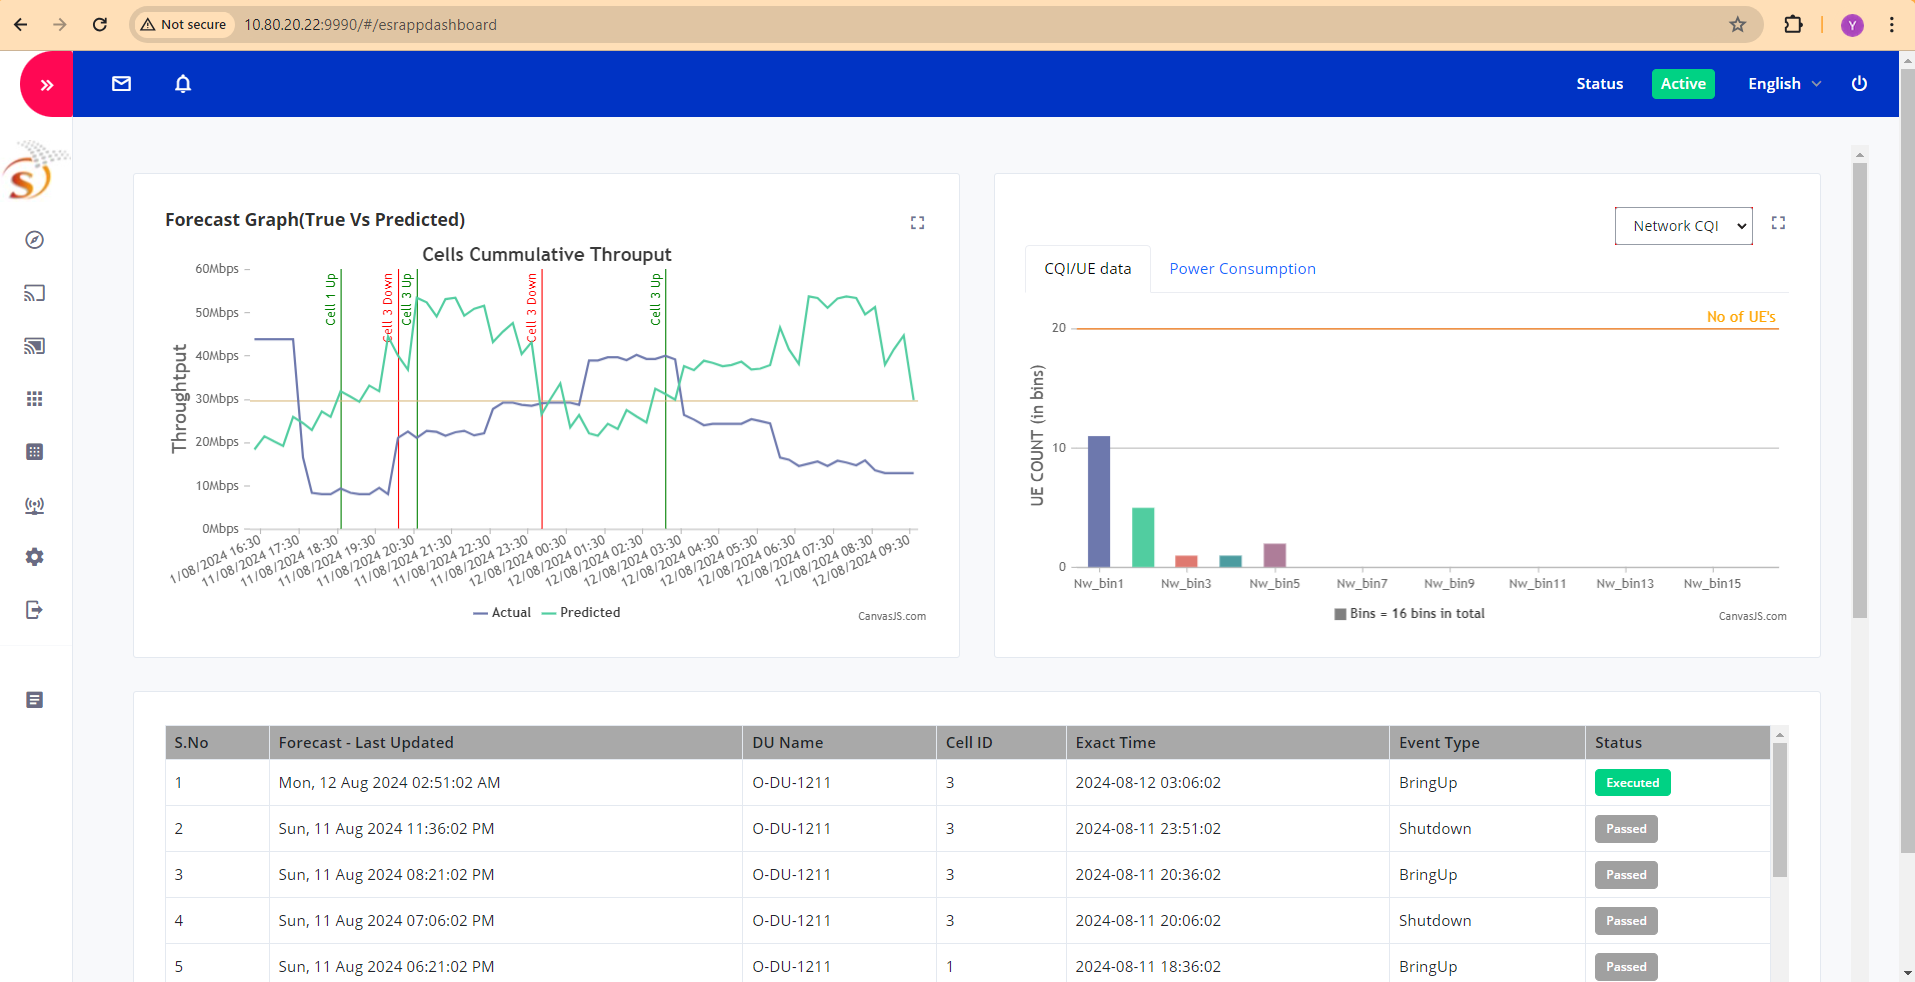
\includegraphics[width=0.4\textwidth]{/Users/pulakmehrotra/Desktop/SaankhyaLabs/es_oran_paper/acm_version_final/images/dashboard.png}
    \caption{ES rApp GUI}
    \label{fig:dashboard}
    \end{figure}

%Space-time partitioning: This is a technique used to divide data based on both spatial (location) and temporal (time) dimensions. In the context of the rApp, this could involve organizing Key Performance Indicators (KPIs) by specific geographical areas (cells, sectors, etc.) and time periods to better manage and analyze the data.
%Continuous time-based aggregation: This refers to the process of continuously collecting and summarizing data over time. Instead of analyzing data at discrete intervals, it is aggregated in a continuous manner, which allows for more fluid and accurate monitoring of KPIs.
%Group KPIs by time: This involves organizing the Key Performance Indicators (KPIs) into groups based on the time they were recorded. This helps in analyzing trends and patterns over specific time periods.
%The standalone application for an ESC node described in 2.2 is connected to the OpenSAS. This application indepen-dently senses the CBRS spectrum for any activity. If activityis detected, it sends IQ data to the model running insidethe OpenSAS for incumbent detection. The current imple-mentation is to detect incumbent (radar) in a 5G New Radio(NR) based CBRS network deployment. Additionally, the re-searchers could use this platform to experiment with theirown models for detecting signals of their interest throughthe ESC node in testbed environments.
%Network traffic prediction has always been a largely explored subject in networking, with a flurry of recent proposals ushered in by the recent development of machine and deep learning tools. Such deep learning-based algorithms have recently been explored to find potential representations of network traffic flows for all types of networks, including Internet, cellular, etc. We first categorize cellular traffic problems into two main types – temporal prediction problems and spatiotemporal prediction problems. Modelling the traffic flow through a node exclusively as a time series is an example of the temporal approach towards network traffic prediction [11]. High traffic on a given node in a cellular network often implies a high load on the other nearby nodes. Taking the traffic flow of nearby nodes and other external factors into consideration when modelling is known as the spatiotemporal approach to network traffic prediction. Spatiotemporal approaches are found to give slightly more accurate forecasts [12].
%Both types of problems can be formulated as supervised learning problems with a difference being in the form of feature representation. In the temporal approach, the collected traffic data can be represented as a univariate time series and the prediction for the values in the future time steps is based on the historical data of the past time steps. In [13], Clemente et Al used Naive Bayes classification and the Holt-Winters method to perform the temporal network forecasting in real time Clemenete et Al first performed systematic preprocessing to reduce bias by selecting the cells with less missing data occurrences, which was then selected to train the classifies to allocate the cells between predictable and non- predictable, taking into account previous traffic forecast error. 
%Building upon the temporal approach, Zhang et al. [14] presented a new technique for traffic forecasting that takes advantage of the tremendous capabilities of a deep convolutional neural network by treating traffic data as images. The spatial and temporal variability of cell traffic is well captured within the dimensions of the images. The experiments show that our proposed model is applicable and effective. Even with the ease of machine learning implementations, regression based models have been found to be fairly accurate, as proven by Yu et Al in [15]. In [15], Yu et Al applied a switching ARIMA model to learn the patterns present in traffic flow series, where the variability of duration is introduced and the sigmoid function describes the relation between the duration of the time series and the transition probability of the patterns. The MGCN-LSTM model, presented in [16] by Len et Al, was a spatial-temporal traffic prediction model which implemented a multi-graph convolutional network (MGCN) to capture spatial features, and a multi-channel long short-term memory (LSTM) to recognise the temporal patterns among short-term, daily, and weekly periodic data. The proposed model was found to greatly outperform commonly implemented algorithms such as ARIMA, LSTM and ConvLSTM.
%Hybrid models can handle a variety of data types and structures, making them ideal for diverse applications along with combining the best features of different methodologies. This very principle is proven by Kuber et Al in [17] which proposes a linear ensemble model composed of three separate sub-models. Each sub-model is used to predict the traffic load in terms of time, space and historical pattern respectively, handling one dimension particularly. Different methodologies such as time series analysis, linear regression and regression tree are applied to the sub-models, which is aggregated and found to perform comparable to a ResNet-based CNN model. Another approach for the same is highlighted in [18] Tian et Al. The approach involves analysing the chaotic property of network traffic by analyzing the chaos characteristics of the network data. [18] proposes a neural network optimization method based on efficient global search capability of quantum genetic algorithm and based on the study of artificial neural networks, wavelet transform theory and quantum genetic algorithm. The proposed quantum genetic artificial neural network model can predict the network traffic more accurately compared to a similarly implemented ARMA model.\\
	
\section{Decision Algorithm}
\label{sec:algorithm}

\subsection{Overview}

The following subsections provide a detailed workflow of the solution discussed in the previous secction, along with an in-depth explanation of the components involved in this decision-making process.
This section provides answers to the challenges outlined in the \hyperref[sec:ps]{Problem Statement}. Each component and its corresponding challenge are discussed in detail.

Within the O-RAN framework, the application manifests as a rApp hosted in Non Realtime RIC and the decision is fed to the xApps and SDNR. 
The data collection and cleaning is done at the edge cloud to take advantage of the distributed processing and avoid pushing large amounts of data to regional data centers.
Firstly, the E2 Nodes are configured by the Service Management and Orchestration (SMO) to report the data necessary via the O1 Interface. 
The functioning of the Non-RT RIC and SMO are tightly coupled, which enables the Non-RT RIC to retrieve the collected data through internal SMO communication. 

In our setup, the rApp receives input data from the Radio Database, Traffic Predictor, and Coverage Predictor, each answering a question posed in \ref{sec:ps}.
The rApp sends a shutdown/bringup policy as a declarative statement, across the A1 interface, to the Near-RT RIC. 
A Traffic Steering xApp assists in the “safe harboring” of users connected to an eNB before shutdown and bringup through the handover process. 
The decision is made periodically, with a 1-hour prediction window and 15-minute slots, i.e., four predictions are made every window. 
The rApp can import data from RF link simulators and drive tests through an external interface. 
A Dashboard for visualization of the system setup is also used with individual components represented in the \hyperref[sec:results]{Results}.

\subsection{Decision Making Entity (DME)}

\subsubsection{Cell Deactivation}

The Decision Making Entity, the cornerstone of our Energy Saving Solution, serves two primary functions: determining whether a cell should be considered for shutdown or bringup, and assessing the consequences of energy-saving decisions prior to modifying the network configuration. 
The decision-making process leverages real-time data and incorporates historical predictions from both the Traffic Predictor and Coverage Predictor.
The entity utilizes short-term throughput forecasts from the Traffic Predictor to determine whether a cell should be considered for shutdown/bringup.
The entity considers shutting down a cell if the throughput exceeds a certain threshold, and conversely, contemplates activating a cell if the throughput falls below this threshold.

After finalizing the decision to either activate or shut down a cell, the Coverage Predictor aids the entity in identifying the network sectors that can be deactivated with minimal service disruption. 
Once the control decision and its target cell are both confirmed, the entity uses the Digital Twin's simulations to assess the potential impact of the energy-saving policy before configuring the network via the SMO.
The overall functioning of this entity is defined in the procedure detailed in \hyperref[alg:energy_saving_algo]{Algorithm 1}.\\

\begin{algorithm} [t!]
    \caption{
        \texttt{Energy Saving Entity Algorithm},
    }
    \begin{algorithmic} [1]
        \Procedure{EnergySavingEntity}{\textsf{$\tau$, curr\_tpt, cqi\_curr, $\alpha_{th}$}}
            \State $\textsf{tpt\_pred} \gets \textsf{TrafficPredictor(curr\_tpt)}$
            \If{$\textsf{tpt\_pred} > \tau$}
                \State \# Cell shutdown procedure
                \State $\textsf{c\_map} \gets \textsf{CoveragePredictor()}$
                \State $\textsf{node} \gets \max(\textsf{c\_map})$ \Comment{Node with maximum $E_{ij}$ for given sector}
                \State Create \textsf{policy} for shutdown.
                \State $\textsf{policy} \gets \textsf{node}$
                \State $\textsf{cqi\_future} \gets \textsf{DigitalTwin(policy)}$
                \State $\alpha \gets \textsf{KL-Divergence}(\textsf{cqi\_future}, \textsf{cqi\_curr})$
                \If{$\alpha < \alpha_{th}$}
                    \State Transmit \textsf{policy}.
                \Else
                    \State Reinvoke \textsf{EnergySavingEntity($\tau$, curr\_tpt, cqi\_curr, $\alpha_{th}$)}.
                \EndIf
            \Else
                \State \# Cell bring-up procedure
                \ForAll{\textsf{nodes} switched off in the system}
                    \State Create \textsf{policy} to switch on node $n$.
                    \State $\textsf{cqi\_n} \gets \textsf{DigitalTwin(policy)}$
                    \State $\alpha_{n} \gets \textsf{KL-Divergence}(\textsf{cqi\_n}, \textsf{cqi\_curr})$
                \EndFor
                \State Select \textsf{finalPolicy} with $\min \left(\textsf{mod}(\alpha_{n} - \alpha_{th})\right)$.
                \State Transmit \textsf{finalPolicy}.
            \EndIf
        \EndProcedure
    \end{algorithmic}
    \label{alg:energy_saving_algo}
\end{algorithm}

\subsection{$\boldsymbol{\Gamma1}$: Traffic Prediction (TP)}
The Traffic Predictor estimates the net traffic volume for each sector as a function of time, helping us decide when would be an potimum  time for shutdown. 
There is no existing technology that can model the traffic in a network with 100\% accuracy. 
This observation is well-established and can be ascribed to the inherent unpredictability of network traffic.
Our approach emphasizes the use of a predictive model to accurately anticipate network traffic \textit{fluctuations}.
We establish a throughput threshold, beyond which network configurations require modification. 
The model is trained with the anticipation that it can guide us towards the appropriate direction of change, accounting for a certain degree of expected error.
To prevent altering our system's configarition based on an erroneous prediction, we use the Digital Twin to simulate the effects of the change before implementing it in the real network.  
We intended to find a regression model that, above all, identified the trend and seasonality of traffic fluctuations.

We use an offline model for learning because using a pre-trained model with sufficient data does seem to suffice to predict traffic directions in our given setup.
%Another reason, we do not use an online model is because traffic data varies irratically and not all the data we recieve is a scenario we want to model for.
In further versions of the solution, we plan to use an online learning model to update the model with real-time data.
Keeping in that in mind, we performed a few experiments with different regression models and found that the LSTM model was the best fit for our requirements.
Although we conducted thorough experiments for model selection and verification, we could not include the details in this paper due to space constraints.

In our solution, this prediction is based on historical data and previous measurements. 
The Traffic Predictor uses a pre-trained LSTM with 64 cells to forecast these values for the near-future. 
The LSTM was trained on on initial system data (initial 300 entries from NS3 simulator), using a batch size of 32 and 100 training epochs. 
The inputs to the LSTM model are throughput, cell to which throughput belongs and the timestamp of the reading.
Every 1 hr, the model makes four fresh predictions (+15, +30, +45, +60).
Based on this, a decision on when cell control is to be implemented is made.

\subsection{$\boldsymbol{\Gamma2}$: Digital Twin (DT)}

The Digital Twin is a powerful tool for network management and optimization, as it allows operators to test and predict the effects of changes of a policy in a risk-free virtual environment before implementing it in a real network.
In the context of our solution, the Digital Twin is used to simulate a cellular network and is used to understand how the cell shutdown/bringup will affect the system overall. 
Our solution utilizes the same validation process to confirm the effectiveness of our policy decisions.

It is implemented using CloudRF \cite{cloudrf}.
The coverage area is represented as a 30 x 30 pixel grid, with power readings simulated for each individual pixel.
CloudRF is used to map out the area of service and simulate the network characteristics across it. 
CloudRF generates predictions of the expected CQI distribution of the system using a Radio Link budget simulator.
This system is initialized with network inventory and predicted RF power (downlink) for each pixel from all sectors in service.

\subsection{$\boldsymbol{\Gamma3}$: Coverage Prediction (CP)}

The Coverage Predictor estimates the \textit{coverage overlap}, the areas where signals from neighboring sectors intersect.
It identifies sectors that, if shut down, would not impact the overall network coverage.
Sectors exhibiting the highest degree of overlap are prioritized for shutdown, given that their discontinuation is less likely to impact coverage due to the compensatory capabilities of the remaining interconnected sectors.

%It also updates the link level prediction model based on actual measured values to enhance accuracy. 
The system takes as input the simulated received power level (sourced from CloudRF) for each pixel from the participating sectors. 
The system outputs a matrix, known as the Coverage Map, which represents the degree of overlap between these sectors. 
The algorithm for the Coverage Predictor is detailed in \hyperref[alg:coverage_algo]{Algorithm 2}.
In the algorithm, $E_{ij}$ represents the number of sectors which have overlaps with other sectors.

\begin{algorithm} [t!]
    \caption{
        \texttt{\sysname pipeline flow}, 
        % \textit{Input:} 
        %     packet \textsf{pkt},
        %     current state \textsf{curr\_state},
        %     current round number \textsf{curr\_rd},
        %     operation mode \textsf{op\_mode},
        % \textit{Output:} 
        %     enncrypted/decrypted pkt \textsf{pkt'} 
    }
        \begin{algorithmic} [1]
            \Procedure{p4ead\_pipeline}{\textsf{pkt}, \textsf{curr\_state}, \textsf{curr\_rd}, \textsf{op\_mode}}
                \State prnd\_count $\gets$ 0
                \While{\textsf{prnd\_count} $<$ \textsf{RPP}} \label{algline:rpp}
                    \If{curr\_state == START}
                        \State curr\_state $\gets$ INIT
                        \State \textsf{pkt} $\gets$ \Call{INIT}{\textsf{pkt}}
                    \ElsIf{curr\_state == INIT}
                        \If{curr\_rd == 12}
                            \State curr\_state $\gets$ ABS\_AD
                            \State \textsf{pkt} $\gets$ \Call{AD\_ABS}{\textsf{pkt}}
                            \State curr\_rd $\gets$ 0
                        \EndIf
                    \ElsIf{curr\_state == ABS\_AD}
                        \If{curr\_rd == 6}
                            \State curr\_state $\gets$ ABS\_IP
                            \State \textsf{pkt} $\gets$ \Call{IP\_ABS}{\textsf{pkt}}
                            \State curr\_rd $\gets$ 0
                        \EndIf
                    \ElsIf{curr\_state == ABS\_IP}
                        \If{curr\_rd == 6}
                            \State curr\_state $\gets$ FINAL
                            \State curr\_rd $\gets$ 0
                        \EndIf
                    \ElsIf{curr\_state == FINAL}
                        \If{curr\_rd == 12}
                            \State curr\_state $\gets$ END
                            \State \textsf{pkt} $\gets$ \Call{TAG}{\textsf{pkt}}
                            \State \Call{break}{}   
                        \EndIf
                    \EndIf
                    \State \textsf{pkt} $\gets$ \Call{p\_rnd}{\textsf{pkt}}  \Comment{do one P-RND}
                    \State prnd\_count $\gets$ prnd\_count $+ 1$
                    \State curr\_rd $\gets$ curr\_rd $+ 1$
                \EndWhile
                \If{curr\_state == END}
                    \If{op\_mode == DECRYPT}
                        \State valid\_tag $\gets$ \Call{verify\_tag}{\textsf{pkt}}
                        \If{$\neg$valid\_tag}
                            \State \Call{drop}{\textsf{pkt}}
                        \EndIf
                    \EndIf
                    \State \textsf{pkt'} $\gets$ \textsf{pkt}
                    \State \Call{forward}{\textsf{pkt'}}
                \Else
                    \State \Call{recirculate}{\textsf{pkt}} 
                \EndIf
            \EndProcedure
        \end{algorithmic}
        \label{alg:pipeline}
    \end{algorithm}
    
     % \If {(cCount - \textsf{cms}.get\_count(flowId)) > $\sigma$} \label{algorithm_access_check_count_start}
     %                \State \textsf{pkt}.ctrl $\gets 0$ \COMMENT{prepare alert}
     %                \State \textsf{pkt}.dst\_ip $\gets$ \Call {Get\_Border\_IP}{\textsf{pkt}.ctrl.borderId}\label{algorithm_access_check_count_end}

       

\subsection{Measuring QoS Gurantees}

In the realm of networking, QoS primarily entails ensuring a specific level of performance for a data flow. 
This is achieved by prioritizing certain network characteristics over others. %\cite{sigcomm}.
In order to uphold QoS commitments in our system, it is essential to ensure that the implementation of energy-saving policies does not lead to a non-trivial decline in network performance.
This can be achieved by ensuring the system operates optimally at the outset and maintaining its initial state throughout. This principle guides our approach to monitoring system functioning.
Among these variables, the \textit{CQI} values of the UEs connected to the active cells and the system's \textit{total throughput} are of paramount importance.

\textit{Why don't we consider the throughput of each individual UE?} Firstly, it's logistically impractical. 
UEs connect and disconnect from the network at a rapid pace, making it difficult and computationally intensive to track individual allotments.
Secondly, as long as the total system performance remains consistent with its state prior to control application, our initial QoS is assured.
Rather than focusing on individual metrics, we concentrate on measuring the system's CQI distribution. 
A low CQI value signifies poor channel quality, while a high CQI value signifies excellent channel quality. 
Our goal is to utilize high-quality channels. By consistently maintaining the use of such channels, we can ensure the preservation of the QoS to the users.

The overall system's CQI is measured by assigning each UE to a CQI-value 'bin', which is determined based on the channel quality measured by the core network.
The distribution of UEs across CQI bins closely mirrors a discrete probability distribution of CQI values across the network.
We employ the Kullback-Leibler (KL) divergence, a statistical measure from information theory, to ensure that the input or output distributions do not deviate significantly from a baseline distribution.
The KL divergence of two probability distributions $P$ and $Q$ is defined as:

\begin{equation}
D_{KL}(P, Q) = \sum_{i} P(i) \log \frac{P(i)}{Q(i)}
\end{equation}
\noindent In this context, $P(i)$ and $Q(i)$ represent the probabilities of the $i$th CQI bin in the respective distributions $P$ and $Q$.

We derive the initial CQI distribution from the NS-3 simulator. 
Subsequently, the rApp policy is applied to generate a new network configuration, which is simulated in the Digital Twin to obtain a subsequent CQI distribution. 
If the control policy doesn't cause a substantial divergence from the baseline in the simulation (quantified using the previously defined KL Divergence), it is subsequently forwarded to the Near-RT RIC.
The user sets the difference threshold, $\alpha_{th}$, which varies based on the specific environment the network is present in.
\section{Design Rationale}
\label{sec:design_rationale}

This section deals with explaining our reasoning and the experiments that lead to the methodology of our solution implementation. 
Initially, we discuss how the decision variables taken for our solution were chosen.
In the later set of experiments, we elucidate our reasoning behind the choice of regression model used to represent the overall network throughput.

\subsection{Decision Variables and Threshold Selection}

The decision-making process in any solution is governed by a set of decision variables that determine the course of action to be taken.
We proceed to evaluate the performance of our Energy Saving solution in terms of the three metrics mentioned below:
\begin{itemize}
  \item \textbf{Network CQI Distribution:} As described in [\textcolor{blue}{CITE}], we categorized the CQI values of the UEs based on the channel quality.
  \item \textbf{Network Throughput:} This metric represents the total throughput used by all the UEs connected to the system.
  \item \textbf{System Power Consumption:} This is the total power consumed by the system, measured in Watts (W).
\end{itemize}

The most important one to consider here is the throughput of the network, which is the primary metric used to decide whether a system needs a change in it's configiration or not.
The rationale behind this is simple: our focus is on the aggregate network performance, and throughput serves as a reliable metric for this purpose.
If the network state, specifically the channel quality and overall throughput, remains largely unchanged after the application of network-modifying policies, we deem the result acceptable.

The determination of thresholds for various decision variables is often crucial to the success of the algorithm. 
In this context, we aim to derive specific expressions to guide the selection of these variables.
In our proposed solutions, we have three primary decision variables: $\tau$, $\alpha_{th}$, and $P_{th}$.
- $\tau$ is the threshhold on the forecasted throughput, which is used to decide whether to shut down a cell or not.
- $\alpha_{th}$ is the allowed divergence of the forecasted/likely CQI distribution from the current CQI distribution. It is used to decide whether a policy should be implemented or not.
- $P_{th}$ is the threshold on the power consumption of the cell. Only cells function above a certain energy-consumption threshold are to be considered for shutdown/bringup.
\\
\textcolor{red}{[PRAMIT] \\
Could you please provide a short write-up on how $\tau$, $\alpha_{th}$ and $P_{th}$ are selected? What are the factors we consider?}

\subsection{Datasets In Use}

The models underwent evaluation using a mix of four real-world and five synthetic time-series datasets, each exhibiting diverse trends and seasonal patterns:

\begin{itemize}
  \item Dataset 1: COMED Dataset - This real-world dataset, sourced from the Commonwealth Edison Company, illustrates the temporal variations in power consumption across a specific group of households.
  \item Dataset 2: Microsoft Dataset - This dataset, obtained using a data scraper, encapsulates the temporal variations in Microsoft's stock price.
  \item Dataset 3: Temperature Dataset - This dataset, sourced from Kaggle, depicts the temporal progression of the Earth's surface temperature.
  \item Dataset 4: No Trend Dataset - This synthetic dataset, created using a blend of sinusoidal and random noise functions, exhibits no discernible trend or seasonality.
  \item Dataset 5: Upwards Trend Dataset - This synthetic dataset is similar to Dataset 4, but it exhibits a noticeable upward trend (without any seasonality).
  \item Dataset 6: Downwards Trend Dataset - This synthetic dataset is similar to Dataset 4, but it exhibits a noticeable downward trend (without any seasonality).
  \item Dataset 7: Upwards Trend Dataset with Seasonality - Dataset 5 with added seasonality.
  \item Dataset 8: Downwards Trend Dataset with Seasonality - Dataset 6 with added seasonality.
  \item Dataset 9: Simulator Dataset - A synthetic dataset generated using our ns-3 simulator, taken to ensure that these models perform with traffic data and not just randomized time-serieses.
\end{itemize}

\subsection{Model Selection}
\begin{table*}[ht]
\caption{Performance of Different Models on Various Synthetic Datasets}
\centering
\resizebox{\textwidth}{!}{%
    \begin{tabular}{|*{3}{>{\centering\arraybackslash}p{0.33\textwidth}|}}
    \hline
    \textbf{Dataset Type} & \textbf{Prophet Performance} & \textbf{LSTM Performance} \\
    \hline
    No Trend, No Seasonality & Does not trend correctly, trends in the opposite direction & Follows trend but does not account for the noise well \\
    \hline
    Upwards Trend, No Seasonality & Steadily trends upwards but not according to the data (underfits) & Follows trend but predicts widely off values when accounting for noise \\
    \hline
    Downwards Trend, No Seasonality & Trends appropriately but underfits, does not recognize dataset intricacies & Recognizes trend and seasonality but produces very inaccurate values due to noise \\
    \hline
    Upwards Trend, With Seasonality & Recognizes trend but not seasonality & Recognizes trend and seasonality well, performs satisfactorily with test data \\
    \hline
    Downwards Trend, With Seasonality & Recognizes trend but not seasonality & Recognizes trend and seasonality but produces very inaccurate values due to noise \\
    \hline
    \end{tabular}%
}
\end{table*}

The choice of regression model used for Traffic Prediction is crucial to the success of the solution.
In this section, we compare the performance of three different regression models: Prophet \textcolor{blue}{[CITE]}, ARIMA, and LSTMs.
We train our models on all our real-world datasets (COMED, Microsoft and Temperature) and evaluate their performance on a validation set of the same dataset.
Our findings can be seen in Table \textcolor{blue}{[CITE]}, with the graphs of our forecasts attached in the \textcolor{blue}{[CITE]}.
We observe that the LSTM model outperforms the other models, capturing the trend and seasonlity of the data the best, which are more prevalent in time-series data.
\subsection{Model Verification}
\begin{table*}[ht]
    \caption{Performance of Different LSTM Models on Various Datasets}
    \centering
    \resizebox{\textwidth}{!}{%
      \begin{tabular}{|*{9}{>{\centering\arraybackslash}p{0.11\textwidth}|}}
        \hline
        \textbf{Dataset/Model} & \textbf{Model 1} & \textbf{Model 2} & \textbf{Model 3} & \textbf{Model 4} & \textbf{Model 5} & \textbf{Model 6} & \textbf{Model 7} & \textbf{Model 8} \\
        \hline
        \textbf{Model 1} & 0.044 & 0.0054 & 0.2507 & 2.0302 & 0.6256 & 1.8354 & 1.186 & 1.1158 \\
        \hline
        \textbf{Model 2} & 0.3358 & 0.2262 & 0.2609 & 0.915 & 0.2613 & 0.855 & 0.486 & 0.4774 \\
        \hline
        \textbf{Model 3} & 0.5695 & 0.7270 & 0.4274 & 1.0624 & 0.3611 & 1.091 & 0.6027 & 0.593 \\
        \hline
        \textbf{Model 4} & 1.0267 & 0.5424 & 0.7875 & 0.5457 & 0.7711 & 1.3335 & 0.6144 & 0.9841 \\
        \hline
        \textbf{Model 5} & 0.5713 & 0.6027 & 0.4731 & 1.069 & 0.2857 & 1.011 & 0.5556 & 0.5418 \\
        \hline
        \textbf{Model 6} & 1.3595 & 1.1141 & 1.3407 & 1.2204 & 0.9841 & 1.2831 & 1.0261 & 1.0280 \\
        \hline
        \textbf{Model 7} & 0.5459 & 0.3503 & 0.2500 & 0.9837 & 0.2005 & 0.9108 & 0.4610 & 0.4590 \\
        \hline
        \textbf{Model 8} & 0.5806 & 0.2504 & 0.1865 & 0.9605 & 0.1640 & 0.8965 & 0.417 & 0.4134 \\
        \hline
      \end{tabular}%
    }
  \end{table*}
  
  

After arriving at using LSTMs as the model of choice for traffic forecasting, we proceed to verify that the model will be able to handle the simulated load using synthetic data.
To verify the robustness of the model's forecasts, we trained the LSTM models using a diverse range of datasets, each exhibiting unique general trends.
For each dataset, we trained a corresponding LSTM model. 
We used Mean Squared Error (MSE) as an evaluation index to evaluate the forecast accuracy of the models.
Subsequently, we cross-validated each model using the remaining datasets.
The MSE values of all the trained models and the datasets in use is described in in Figures \textcolor{blue}{[CITE]}.
We observe that the LSTM trained on data with more seasonlity (model 7,8 and 9) perform the best all around, with the lowest MSE values.
This is expected, as the LSTM model is designed to capture the long-term dependencies in the data, which are more prevalent in datasets with seasonality.
  
Therefore, when training our model on real-world data, we should ensure that the data has a significant amount of seasonality to ensure the best performance.  
The amount data used to train the LSTM model is crucial to the success of the solution.
If we train the model on excessive data, the model may overfit to the training data and fail to generalize to unseen data.
This will depend on the deployemnt environment's complexity, and in our specific setup we found 300 samples to suffice.


\section{Performance Evaluation}
\label{sec:results}

In this section, we evaluate the performance of our proposed Energy Saving solution in our software-defined O-RAN network. 
Our setup is lightweight, focusing primarily on evaluating the effectiveness of our proposed algorithm rather than the performance of the underlying simulations.
We first discuss the simulation setup, followed by the threshold selection process of various decision variables. 
Our experiments to prove the effectiveness of the proposed algorithm are then presented, followed by a discussion on maintaining QoS guarantees.
In the ensuing graphs, to illustrate the long-term impact of the energy-saving algorithm, we've adopted a time conversion convention where 10 seconds equate to 15 minutes. 

\subsection{Simulation Setup}
Our solution is deployed as an independent rApp, interfacing with the Non-RT RIC and the A1 interface of the O-RAN stack. 
This rApp dispatches decision-making policies to the Near-RT RIC, which houses the TS xApp responsible for reallocating UEs during cell shutdown or bringup processes.
The network, simulated as a Digital Twin using an NS-3 Simulator, comprises eight cells with 20 User Equipments (UEs) per cell, operating in a single-threaded mode.
The rApp operates in a feedback loop with the Digital Twin, obtaining power readings, throughput, and other characteristics across the coverage area.
\textcolor{red}{The network is configured to operate in a 5G New Radio (NR) based CBRS network deployment.}

The Digital Twin in use here is a different one as the one mentioned earlier in the paper in the Algo section \textcolor{blue}{[CITE]}.
The Digital Twin integrated into the ES rApp, is a streamlined simulator that reports selected characteristics of the deployed system, implemented using CloudRF.
The NS-3 simulator serves as the backbone for our network simulation, encompassing the core network, the gNBs, and the UEs. 
The Digital Twin, as previously described, supplements this setup by furnishing the rApp with requisite data.
A more comprehensive explanation of the Digital Twin setup can be provided in the Appendix. [\textcolor{blue}{CITE}]

\subsection{Power Consumption Reduction}

As described in \textcolor{blue}{[CITE]}, the proposed algorithm ensures that the QoS guarantees are maintained during the cell shutdown and bringup processes.
We try to ensure the policy proposed does not lead to a significant drop in the overall CQI of the channels in use for transmission.
We have conducted a series of experiments to evaluate the performance of our proposed solution especially considering the reduction in the power consumption over the given .
First, we look at the performance figures on how the forecasts of the overall throughput help achieve cell shutdown and bringup.

\textcolor{red}{[YOGESH] \\
What is the experiment we are performing? --> A simulation over a certain time-frame, which shows:\\
- Throughput increase or decrease leads to cell shutdown or bringup.\\
- How the power consumption of the system decreases over time.\\
- How the CQI/UE distribution is maintained for atleast a given timeframe \\.
I would like if the first two can be be compared vertically, with time stamps for cell shutdown/bringup maintained. 
The second graph can simply be a comparision of the CQI distribution at the start and the end of the experiment.}

\subsection{Maintaining QoS Guarantees}
\textcolor{red}{[YOGESH] \\
We can view the results in Fig 3. for Cell Shutdown and Bringup both.
Fig 4. shows how our given solution leads to an eventual decrease in total power consumption of the system.
Fig 5. (right now Fig. 2) shows how the CQI distribution is maintained over the given time-frame.}

\begin{figure}[ht]
  \centering
  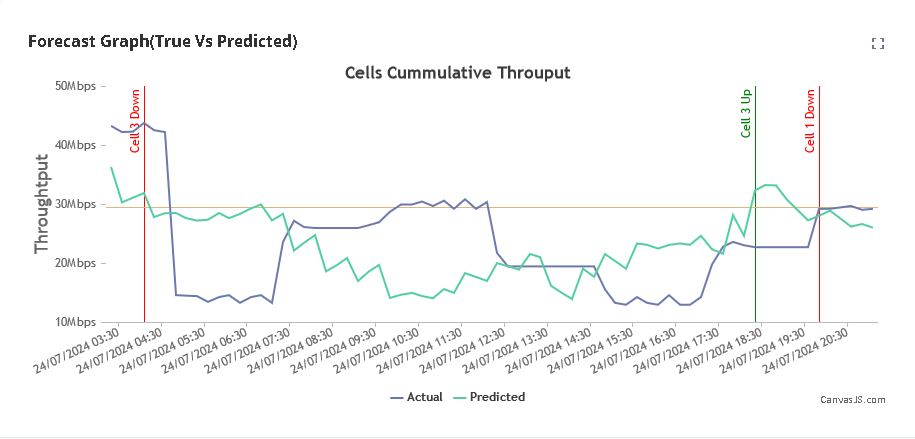
\includegraphics[width=0.4\textwidth]{/Users/pulakmehrotra/Desktop/SaankhyaLabs/es_oran_paper/acm_version_final/images/tpt.png}
  \caption{Throughput Forecasts and Decision Making}
  \label{fig:tpt}
  \end{figure}

\begin{figure}[ht]
  \centering
  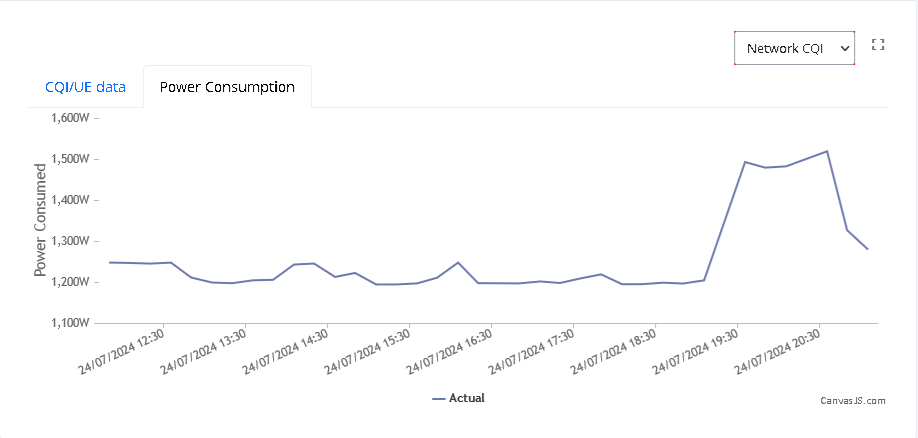
\includegraphics[width=0.4\textwidth]{/Users/pulakmehrotra/Desktop/SaankhyaLabs/es_oran_paper/acm_version_final/images/power_consumption.png}
  \caption{Example of Energy Saving Results}
  \label{fig:power}
  \end{figure}



\section{Conclusion and Future Work}
This work aimed to develop and evaluate an Energy Saving rApp for the O-RAN architecture using decision making algorithms and LSTMs for prediction. A LSTM neural network model was trained on various time-series datasets \textcolor{blue}{generated using the NIST radar (incum-bent) waveform generator}. Also, 5G NR data was capturedusing the ESC sensor node with the SDR based CBSD asthe signal source. The collected 5G NR data was mixed withthe NIST generated datasets to train the ML model for 5GNR non-incumbent detection. The model training resultsshow better performance at higher SNR values as expected.The highest prediction accuracy of 95.83\% was achieved for \textcolor{blue}{[PULAK - Edit in the end] dataset with signals in the SNR range 40-50 dB}. OTA incum-bent detection is achieved by transmitting the signals in thedataset OTA and results are presented. In the OTA resultsfor incumbent detection, the highest accuracy achieved is 85.35\%. Additionally, the results for the OTA non-incumbent(5G-NR) signal is presented. The model achieves an accuracyof 91.3% for OTA non-incumbent detection.

The energy saving results via ML-enabled rApp control in the the simulated NS-3 environment are encouraging and provide a basis for further enhancement in the ML model as well as the decision-making entity to incorporate other decision variables as the future scope of the work. Also, other prediction models can be implemented to analyze different model performances in the end-to-end experimental deployment. Furthermore, the enhanced rApp version provides an overall energy-saving solution to be used for efficient RAN control/management, not only in experimental simulations but also in any real-world environment.



\clearpage 

\bibliographystyle{ACM-Reference-Format}
\bibliography{main}

\clearpage
\appendix
\newpage

\section{Coverage Algorithm}
\label{sec:coverage_algo}

\begin{algorithm} [t!]
    \caption{
        \texttt{\sysname pipeline flow}, 
        % \textit{Input:} 
        %     packet \textsf{pkt},
        %     current state \textsf{curr\_state},
        %     current round number \textsf{curr\_rd},
        %     operation mode \textsf{op\_mode},
        % \textit{Output:} 
        %     enncrypted/decrypted pkt \textsf{pkt'} 
    }
        \begin{algorithmic} [1]
            \Procedure{p4ead\_pipeline}{\textsf{pkt}, \textsf{curr\_state}, \textsf{curr\_rd}, \textsf{op\_mode}}
                \State prnd\_count $\gets$ 0
                \While{\textsf{prnd\_count} $<$ \textsf{RPP}} \label{algline:rpp}
                    \If{curr\_state == START}
                        \State curr\_state $\gets$ INIT
                        \State \textsf{pkt} $\gets$ \Call{INIT}{\textsf{pkt}}
                    \ElsIf{curr\_state == INIT}
                        \If{curr\_rd == 12}
                            \State curr\_state $\gets$ ABS\_AD
                            \State \textsf{pkt} $\gets$ \Call{AD\_ABS}{\textsf{pkt}}
                            \State curr\_rd $\gets$ 0
                        \EndIf
                    \ElsIf{curr\_state == ABS\_AD}
                        \If{curr\_rd == 6}
                            \State curr\_state $\gets$ ABS\_IP
                            \State \textsf{pkt} $\gets$ \Call{IP\_ABS}{\textsf{pkt}}
                            \State curr\_rd $\gets$ 0
                        \EndIf
                    \ElsIf{curr\_state == ABS\_IP}
                        \If{curr\_rd == 6}
                            \State curr\_state $\gets$ FINAL
                            \State curr\_rd $\gets$ 0
                        \EndIf
                    \ElsIf{curr\_state == FINAL}
                        \If{curr\_rd == 12}
                            \State curr\_state $\gets$ END
                            \State \textsf{pkt} $\gets$ \Call{TAG}{\textsf{pkt}}
                            \State \Call{break}{}   
                        \EndIf
                    \EndIf
                    \State \textsf{pkt} $\gets$ \Call{p\_rnd}{\textsf{pkt}}  \Comment{do one P-RND}
                    \State prnd\_count $\gets$ prnd\_count $+ 1$
                    \State curr\_rd $\gets$ curr\_rd $+ 1$
                \EndWhile
                \If{curr\_state == END}
                    \If{op\_mode == DECRYPT}
                        \State valid\_tag $\gets$ \Call{verify\_tag}{\textsf{pkt}}
                        \If{$\neg$valid\_tag}
                            \State \Call{drop}{\textsf{pkt}}
                        \EndIf
                    \EndIf
                    \State \textsf{pkt'} $\gets$ \textsf{pkt}
                    \State \Call{forward}{\textsf{pkt'}}
                \Else
                    \State \Call{recirculate}{\textsf{pkt}} 
                \EndIf
            \EndProcedure
        \end{algorithmic}
        \label{alg:pipeline}
    \end{algorithm}
    
     % \If {(cCount - \textsf{cms}.get\_count(flowId)) > $\sigma$} \label{algorithm_access_check_count_start}
     %                \State \textsf{pkt}.ctrl $\gets 0$ \COMMENT{prepare alert}
     %                \State \textsf{pkt}.dst\_ip $\gets$ \Call {Get\_Border\_IP}{\textsf{pkt}.ctrl.borderId}\label{algorithm_access_check_count_end}

       

\section{Dashboard GUI}
\label{sec:dashboard}

\begin{figure}[ht]
  \centering
  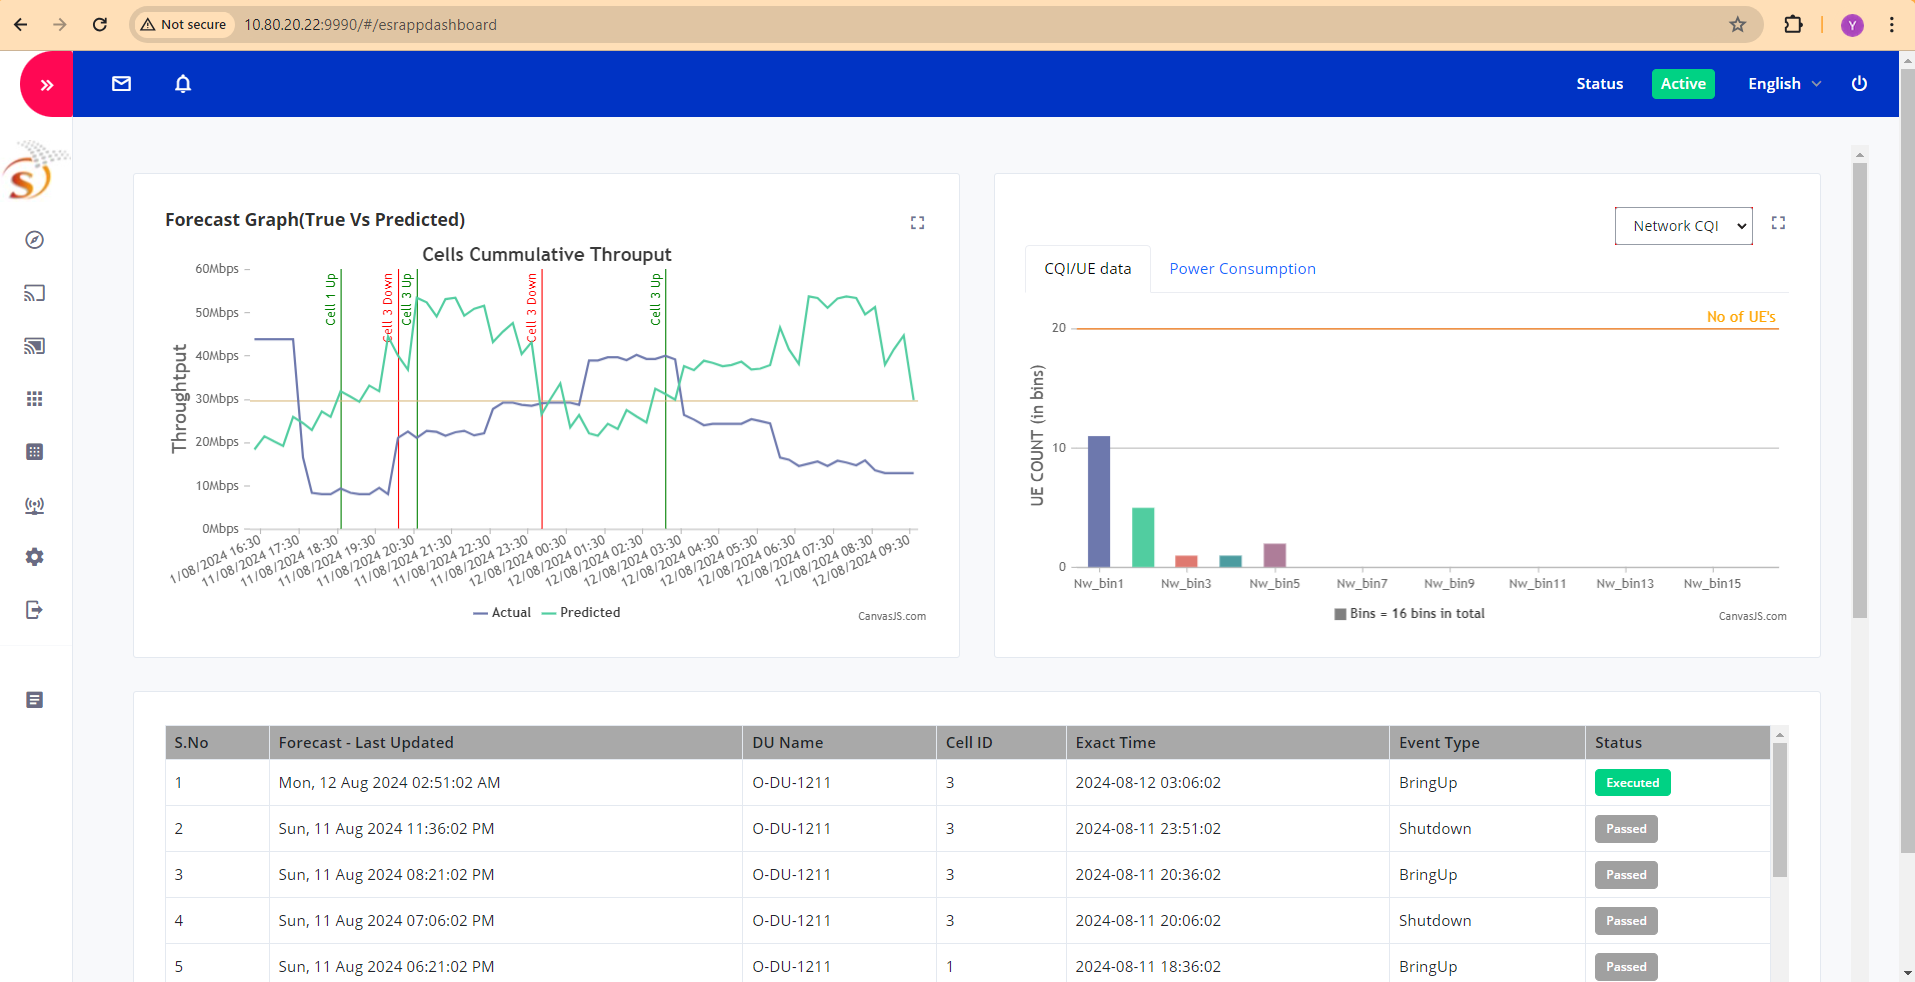
\includegraphics[width=0.5\textwidth]{/Users/pulakmehrotra/Desktop/SaankhyaLabs/es_oran_paper/acm_version_final/images/dashboard.png}
  \caption{ES rApp GUI}
  \label{fig:dashboard}
\end{figure}

\section{Design Rationale}
\label{sec:design_rationale}

In this section, we elucidate our reasoning behind the choice of regression model used to represent the overall network throughput.

\begin{comment}
\subsection{Decision Variables and Threshold Selection}

The decision-making process in any solution is governed by a set of decision variables that determine the course of action to be taken.
We proceed to evaluate the performance of our Energy Saving solution in terms of the three metrics mentioned below:
\begin{itemize}
  \item \textbf{Network CQI Distribution:} As described in [\textcolor{blue}{CITE}], we categorized the CQI values of the UEs based on the channel quality.
  \item \textbf{Network Throughput:} This metric represents the total throughput used by all the UEs connected to the system.
  \item \textbf{System Power Consumption:} This is the total power consumed by the system, measured in Watts (W).
\end{itemize}

The most important one to consider here is the throughput of the network, which is the primary metric used to decide whether a system needs a change in it's configiration or not.
The rationale behind this is simple: our focus is on the aggregate network performance, and throughput serves as a reliable metric for this purpose.
If the network state, specifically the channel quality and overall throughput, remains largely unchanged after the application of network-modifying policies, we deem the result acceptable.

The determination of thresholds for various decision variables is often crucial to the success of the algorithm. 
In this context, we aim to derive specific expressions to guide the selection of these variables.
In our proposed solutions, we have three primary decision variables: $\tau$, $\alpha_{th}$, and $P_{th}$.
- $\tau$ is the threshhold on the forecasted throughput, which is used to decide whether to shut down a cell or not.
- $\alpha_{th}$ is the allowed divergence of the forecasted/likely CQI distribution from the current CQI distribution. It is used to decide whether a policy should be implemented or not.
- $P_{th}$ is the threshold on the power consumption of the cell. Only cells function above a certain energy-consumption threshold are to be considered for shutdown/bringup.
\\
\textcolor{red}{[PRAMIT] \\
Could you please provide a short write-up on how $\tau$, $\alpha_{th}$ and $P_{th}$ are selected? What are the factors we consider?}
\end{comment}

\subsection{Datasets In Use}

We intended to find a regression model that, above all, identified the trend and seasonlity of traffic fluctuations.
The models underwent evaluation using a mix of four real-world and five synthetic time-series datasets, each exhibiting diverse trends and seasonal patterns:

\begin{itemize}
  \item Dataset 1: COMED Dataset - This real-world dataset, released by the Commonwealth Edison Company, illustrates the temporal variations in power consumption across a specific group of households.
  \item Dataset 2: Microsoft Dataset - This dataset, obtained using a data scraper, encapsulates the temporal variations in Microsoft's stock price.
  \item Dataset 3: Temperature Dataset - This dataset, sourced from Kaggle, depicts the temporal progression of the Earth's surface temperature.
  \item Dataset 4: No Trend Dataset - This synthetic dataset, created using a blend of sinusoidal and random noise functions, exhibits no discernible trend or seasonality.
  \item Dataset 5: Upwards Trend Dataset - This synthetic dataset is similar to Dataset 4, but it exhibits a noticeable upward trend (without any seasonality).
  \item Dataset 6: Downwards Trend Dataset - This synthetic dataset is similar to Dataset 4, but it exhibits a noticeable downward trend (without any seasonality).
  \item Dataset 7: Upwards Trend Dataset with Seasonality - Dataset 5 with added seasonality.
  \item Dataset 8: Downwards Trend Dataset with Seasonality - Dataset 6 with added seasonality.
  \item Dataset 9: Simulator Dataset - A synthetic dataset generated using our ns-3 simulator, taken to ensure that these models perform with traffic data and not just randomized time-serieses.
\end{itemize}

\subsection{Model Selection}
\begin{table*}[ht]
\caption{Performance of Different Models on Various Synthetic Datasets}
\centering
\resizebox{\textwidth}{!}{%
    \begin{tabular}{|*{3}{>{\centering\arraybackslash}p{0.33\textwidth}|}}
    \hline
    \textbf{Dataset Type} & \textbf{Prophet Performance} & \textbf{LSTM Performance} \\
    \hline
    No Trend, No Seasonality & Does not trend correctly, trends in the opposite direction & Follows trend but does not account for the noise well \\
    \hline
    Upwards Trend, No Seasonality & Steadily trends upwards but not according to the data (underfits) & Follows trend but predicts widely off values when accounting for noise \\
    \hline
    Downwards Trend, No Seasonality & Trends appropriately but underfits, does not recognize dataset intricacies & Recognizes trend and seasonality but produces very inaccurate values due to noise \\
    \hline
    Upwards Trend, With Seasonality & Recognizes trend but not seasonality & Recognizes trend and seasonality well, performs satisfactorily with test data \\
    \hline
    Downwards Trend, With Seasonality & Recognizes trend but not seasonality & Recognizes trend and seasonality but produces very inaccurate values due to noise \\
    \hline
    \end{tabular}%
}
\end{table*}

The choice of regression model used for Traffic Prediction is crucial to the success of the solution.
In this section, we compare the performance of three different regression models: Prophet, ARIMA, and LSTMs.
We train our models on all our real-world datasets (COMED, Microsoft and Temperature) and evaluate their performance on a validation set of the same dataset.
Our findings can be seen in \hyperref[tab:model_comp]{Table 1}.
We observe that the LSTM model outperforms Prophet, capturing the trend and seasonlity of the data the best.
The ARIMA model was found to be outright the worst performer, both taking the longest to train as well making forecasts completely ignoring the trend and seasonlity of the inputed data.
Considering how promising the LSTM's performance seemed, we decided to further evaluate the same.

\subsection{Model Verification}
\begin{table*}[ht]
    \caption{Performance of Different LSTM Models on Various Datasets}
    \centering
    \resizebox{\textwidth}{!}{%
      \begin{tabular}{|*{9}{>{\centering\arraybackslash}p{0.11\textwidth}|}}
        \hline
        \textbf{Dataset/Model} & \textbf{Model 1} & \textbf{Model 2} & \textbf{Model 3} & \textbf{Model 4} & \textbf{Model 5} & \textbf{Model 6} & \textbf{Model 7} & \textbf{Model 8} \\
        \hline
        \textbf{Model 1} & 0.044 & 0.0054 & 0.2507 & 2.0302 & 0.6256 & 1.8354 & 1.186 & 1.1158 \\
        \hline
        \textbf{Model 2} & 0.3358 & 0.2262 & 0.2609 & 0.915 & 0.2613 & 0.855 & 0.486 & 0.4774 \\
        \hline
        \textbf{Model 3} & 0.5695 & 0.7270 & 0.4274 & 1.0624 & 0.3611 & 1.091 & 0.6027 & 0.593 \\
        \hline
        \textbf{Model 4} & 1.0267 & 0.5424 & 0.7875 & 0.5457 & 0.7711 & 1.3335 & 0.6144 & 0.9841 \\
        \hline
        \textbf{Model 5} & 0.5713 & 0.6027 & 0.4731 & 1.069 & 0.2857 & 1.011 & 0.5556 & 0.5418 \\
        \hline
        \textbf{Model 6} & 1.3595 & 1.1141 & 1.3407 & 1.2204 & 0.9841 & 1.2831 & 1.0261 & 1.0280 \\
        \hline
        \textbf{Model 7} & 0.5459 & 0.3503 & 0.2500 & 0.9837 & 0.2005 & 0.9108 & 0.4610 & 0.4590 \\
        \hline
        \textbf{Model 8} & 0.5806 & 0.2504 & 0.1865 & 0.9605 & 0.1640 & 0.8965 & 0.417 & 0.4134 \\
        \hline
      \end{tabular}%
    }
  \end{table*}
  
  

After arriving at using LSTMs as the model of choice for traffic forecasting, we had to ensure that the model would be able to handle the simulated load. 
We did so using synthetic data of various types, as outlined in our Dataset section.
To verify the robustness of the model's forecasts, we trained the LSTM models using a diverse range of datasets, each exhibiting unique general trends.
For each dataset, we trained a corresponding LSTM model. 
We used Mean Squared Error (MSE) as an evaluation index to evaluate the forecast accuracy of the models.
Subsequently, we cross-validated each trained model with the remaining datasets.
The MSE values of all the trained models and the datasets in use is described in in \hyperref[tab:lstm_performance]{Table 2}.
We observe that the LSTM trained on data with more seasonlity (model 7,8 and 9) perform the best all around, with the lowest MSE values.
This is expected, as the LSTM model is designed to capture the long-term dependencies in the data, which are more prevalent in datasets with seasonality.
  
Therefore, when training our model on real-world data, we should ensure that the data has a significant amount of seasonality to ensure the best performance.  
The amount of data used to train the LSTM model is crucial to the success of the solution.
If we train the model on excessive data, the model may overfit to the training data and fail to generalize to unseen data.
This would be especially catastrophic in our specific use case, as we
This will depend on the deployemnt environment's complexity, and in our specific setup we found 300 samples to suffice.



\end{document}